









\newpage
\subsubsection*{Torsionspendel mit Hantel}
Hier wurde die Schwingungsdauer einer Hantel mit aufgelegten Scheiben beobachtet, wobei der Abstand $a$ des Scheibenschwerpunktes zur Rotationsachse variiert wurde. 



\begin{table}[h]
	\centering	
	\caption{Messdaten des Torsionspendels mit Hantel und aufgelegten Scheiben  }
	\begin{tabular}{|l|c|} 
		\hline 
		Messgröße	& Messwert  \\ 
		\hline 
		Länge des Drahtes $L_D$& \SI{1.8150\pm 0.0004 } {m} \\ 
		\hline 
		Masse der Achse $m_1$& \SI{0.21773}{kg} \\ 
		\hline 
		Radius der Achse $R_1$ & \SI{0.0599 \pm 0.0004}{m}  \\ 
		\hline 
		Länge der Achse $H_1$ &	\SI{0.27\pm 0.0004}	{\metre}	\\
		\hline
		Radius des Drahtes $R_D$ & \SI{2.50+-0.002 e-4} {m} \\ 
		\hline 
		Masse der aufgelegten Scheibe $m_2$& \SI{0.29728}{kg} \\ 
		\hline 
		Radius der aufgelegten Scheibe $R_2$ & \SI{0.0245 \pm 0.0004}{m}  \\ 
		\hline 
		Höhe der aufgelegten Scheibe $H_2$ &\SI{0.0204\pm0.00004 }{\metre}			\\
		\hline
	
	\end{tabular} 
	
	\label{tab:dataTH}
\end{table} 




\begin{figure}[h]
	\centering
	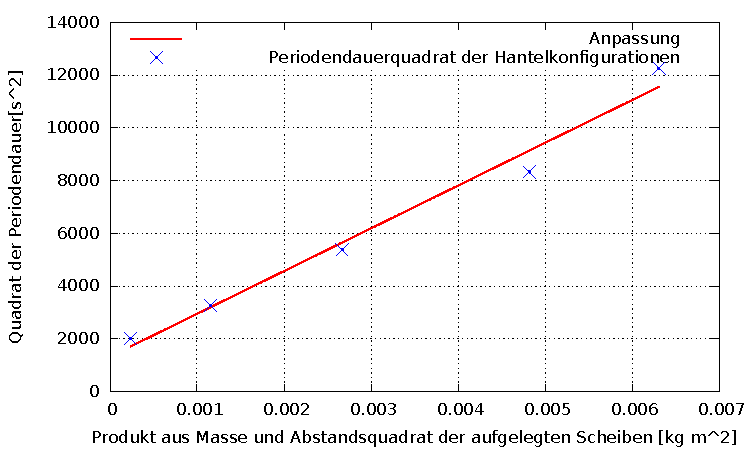
\includegraphics[width=0.7\linewidth]{auswertung/hantel/HantelD}
	\caption{Dargestellt werden die Messung mit Anpassung der Schwingungsdauern der Hantel mit aufgelegten Scheiben in verschiedenen Abständen zur Rotationsachse. Die Einheiten der Achsen sind so gewählt, dass die Messpunkte nach dem Steinerschen Satz linear sind.  }
	\label{fig:hantel}
\end{figure}

Der Steinersche Satz sagt einen linearen Zusammenhang für \cref{fig:hantel} vorher, daher wurde eine Anpassung des Typs $T^2(2m_2 a^2)=b (2m a^2)+c$ gewählt und man erhält nach der Anpassung\footnote{Die Anpassung wurde durch "Gnuplot" mit dem Levenberg–Marquardt Algorithmus vorgenommen.  } die Werte: $ b               = \SI{1.62   \pm 0.13 e+006}{\second \squared \per \kilogram \per \metre \squared} $ und $c               = \SI{ 1.3      +-0.5e3 }   {\second \squared}$. Aus der Steigung $b$ und Gleichung \ref{eq:hantelta} folgt durch Koeffzientenvergleich $D^*=\SI{2.4+-0.2e-5}{\kilogram \metre \squared \per \second \squared }$

%D^* exacter 0.0000243432

%D^* aus 30 ist 0.000266??

%Fit daten
%b               = 1.62174e+006     +/- 1.316e+005   (8.117%)
%c               = 1322.21          +/- 497.8        (37.65%)

%t_p

\begin{align}
	T^2= \frac{4 \pi^2}{D^*}(J_1+2J_2+2m_2 a^2)
	\label{eq:hantelta}
\end{align}



Die Schwingungsdauer der Hantel ohne Scheiben $T_0$  betrug \SI{39,03 \pm 0.08}{s}. Es folgt mit Gleichung \ref{eq:hantelJ} für das Trägheitsmoment des Hantelstabes $J_1 = \SI{9.4 \pm 0.8 e-4}{\kilogram \metre \squared}$.



\begin{align}
	J=\frac{T^2 D^*}{4 \pi^2} \pm \frac{T^2 D^*}{4 \pi^2} \sqrt{
	\left(\frac{2 \Delta T}{T} \right)^2 + 	\left(\frac{2 \Delta D^*}{D^*} \right)^2 }
\label{eq:hantelJ}
\end{align}








Aus dem Parameter $c$ und der Gleichung \ref{eq:hantelta} und $a=0$  folgt für das Trägheitsmoment der Hantelscheiben mit Schwerpunkt auf der Rotationsachse:
\begin{align}
J_2=\frac{c D^*}{8 \pi ^2}-\frac{J_1}{2} \pm \sqrt{\left( \frac{c D^*}{8 \pi}\right) ^2\left( \left( \frac{\Delta c}{c}\right) ^2+  \left( \frac{\Delta D^*}{D^*}\right) ^2\right) + \left(\frac{J_1}{2}\right)^2 }
\end{align}
Es folgt $J_2=\SI{-7.485 \pm 42.9 e-5 }{\kilogram \metre \squared}$ da die Unsicherheit größer als der Wert ist, ist es nicht sinnvoll weitere Betrachtungen mit diesen Werten 




















\newpage


\subsection{Diskussion}

%vgl mit lit wert am ehesten $\alpha$ Eisen $G=\SI{8.4 e9}{kg \per \metre \second \squared}$ abweichungen groß nicht aufgeführte legierung
Im Vergleich mit den Literaturwerten erscheint eine Stahllegierung wahrscheinlich. So besitzt zum Beispiel "CrV-Federstahl" oder "V2A-Stahl" ein Schubmodul\footnote{entnommen: Gerthsen Physik, Vogel 1977} $G=\SI{8.000 e10}{kg \per  \second \squared \metre}$.
Genauso Wahrscheinlich sind jedoch auch andere Stahllegierungen, da die Eigenschaften von den genauen Anteilen der Legierungsbestandteilen steuerbar sind und das gewünschte Schubmodul mit verschiedenen Zusätzen erreicht werden kann.








